\documentclass{article}
% Glyph origins (DESIGN 4.4, `PARTEX_ORIGINS=1`): xtask's `glyphs` job
% checks the origin of each glyph against this text and the PDF's
% content streams. Text, ligatures, a macro, \thesection, hyphenated
% line breaks, a TikZ node, a reused \savebox, a form drawn twice, a
% literal's text, an included PDF page with text, a second page.
\usepackage{tikz}
\usepackage{graphicx}
\newcommand\foo{bar}
\newsavebox\keep
\begin{document}
\section{Intro}
Hello world, first finer office.
A macro: \foo{} and section \thesection.
\savebox\keep{Saved}\usebox\keep{} and \usebox\keep.


\begin{tikzpicture}\node[draw] {Tikz};\end{tikzpicture}

\parbox{4em}{\hspace{0pt}characteristically representative}

\setbox0\hbox{Form}\immediate\pdfxform0
\pdfrefxform\pdflastxform{} twice \pdfrefxform\pdflastxform{} done.
\pdfliteral{BT 3 Tr (lit) Tj ET}After literal.

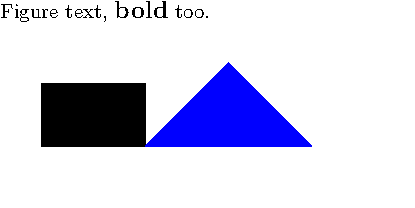
\includegraphics[width=3cm]{images-fig}

\newpage
Second page.
\end{document}
